\chapter{Experiments}

    \section{V1}

        \subsection{Spark ignition}
            
            As was discussed in \cite{duplayArgonLaserPlasmaThruster2024a}, spark ignition was not reliable enough with the available electrode system. 

        \subsection{Bringing the pulsed power down and Optical design (move to design)} \label{sec:design_optics}
            
            Pulsed shots at lower power levels revealed a difficulty to ignite the LSP below \qty{20}{\%} power, which corresponds to about \qty{620}{W}. This poses a problem, as the maximum CW power of the laser is significantly lower, at \qty{350}{W}. A test campaign was started in February 2024 to determine if LSP ignition in the V1 thruster was possible under this maximum CW power level.
            
            To obtain LSP ignition, a high enough laser flux is needed. With a fixed power, it is necessary to focus the laser down to the smallest area possible to get the highest flux. Quantifying the diameter of this focus was therefore the first step. 

            %Section on quantifying diameter, laser optics basics (email from thorlabs guy)

            For a multi-element system, the spot diameter must be calculated numerically with ray tracing software. WinLens 3D Basic \cite{winlens} was used here, as it is free and powerful enough for this application. The single element system was also simulated in this software to verify the calculations.

            Now that the diameter of the focus is known, two avenues are possible to improve it: a shorter focal length or a multi-lens system \cite{thorlabs}. At first, a single lens with a \qty{125}{mm} focal length (Thorlabs LA1384-C \cite{125mm lens}) was used, as it was the simpler option. During these shots, the goal was to achieve LSP ignition at or below \qty{11}{\%} pulsed power, or \qty{340}{W}. The following graph shows LSP ignition attempts at various power settings and axial lens positions. 20 pulsed laser shots were performed for each point on the graph. If at least one was successful at igniting LSP, it was recorded as such. This graph can also be interpreted as a beam profiling for LSP conditions.
            
            % Graph of 125mm lens
            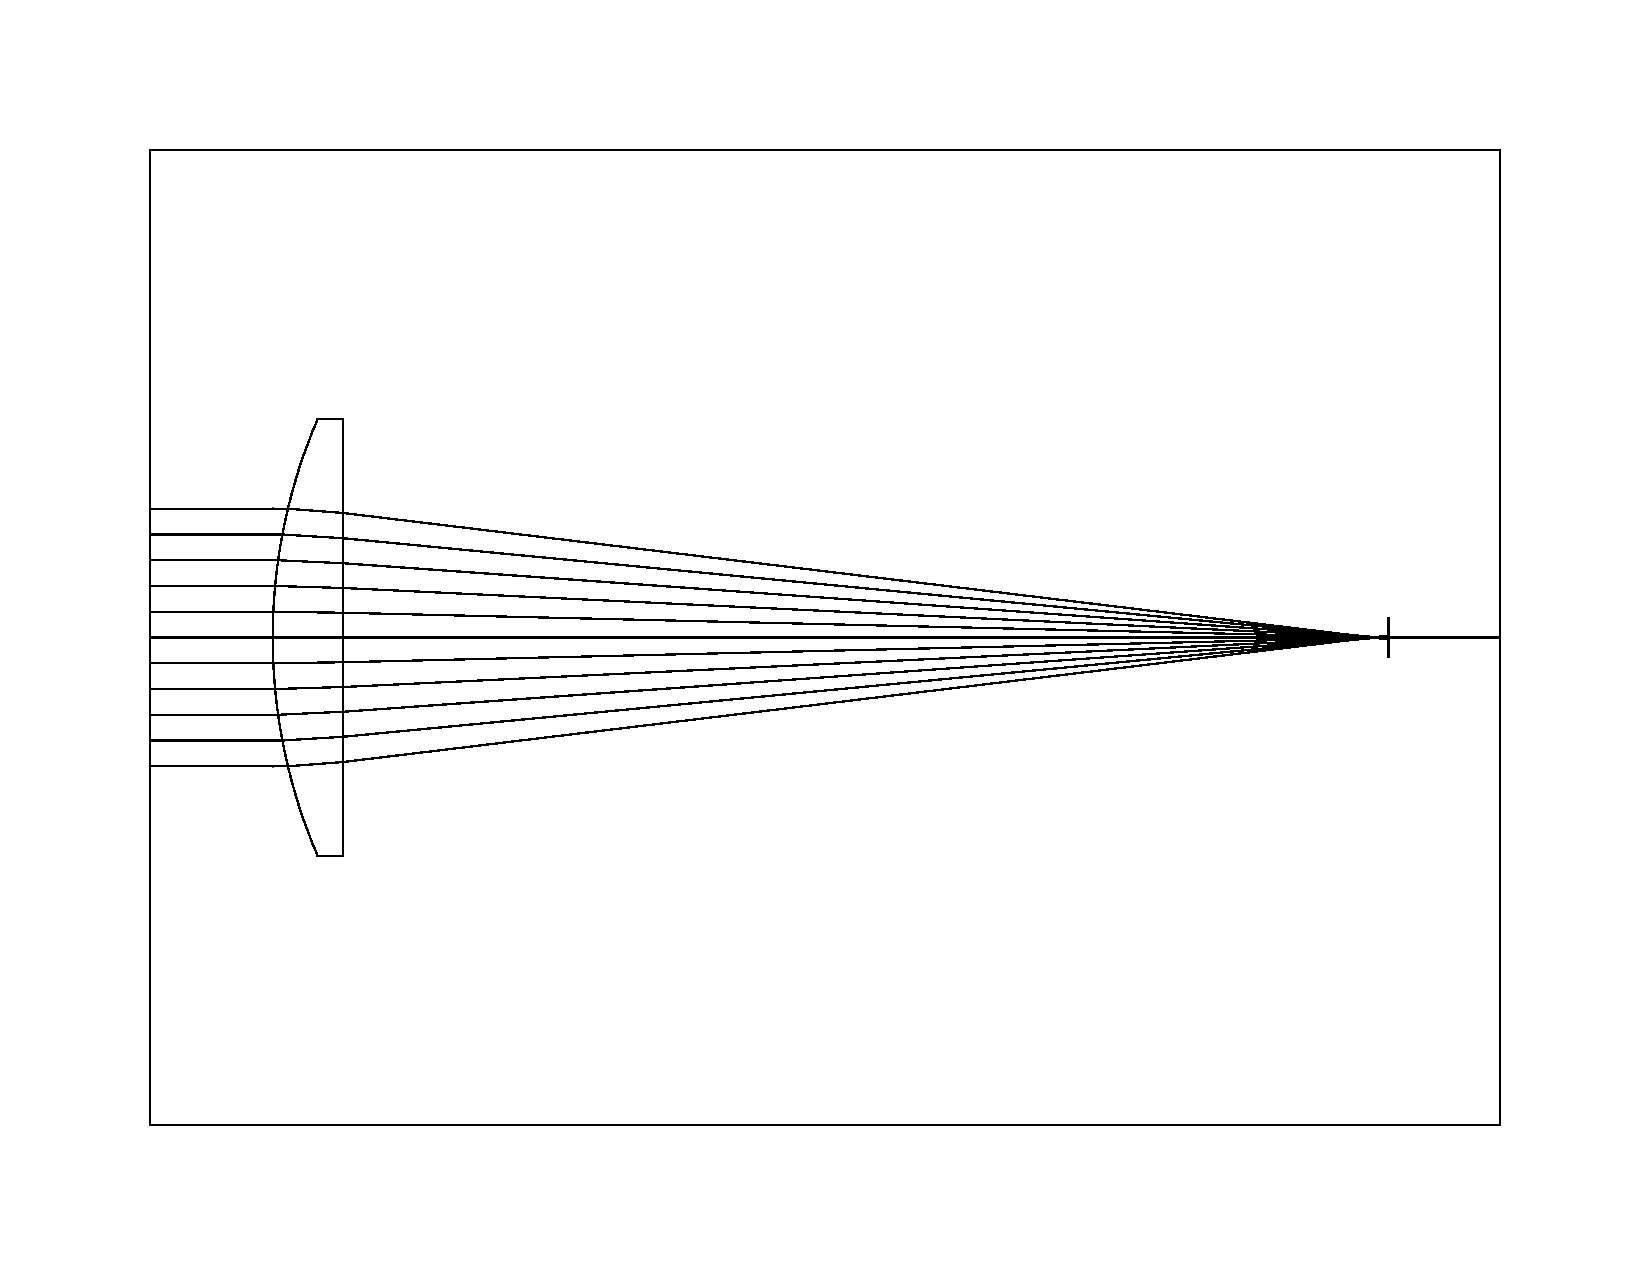
\includegraphics[width=\textwidth]{assets/5 results/125lens.pdf}

            \begin{figure}[h]
                \centering
                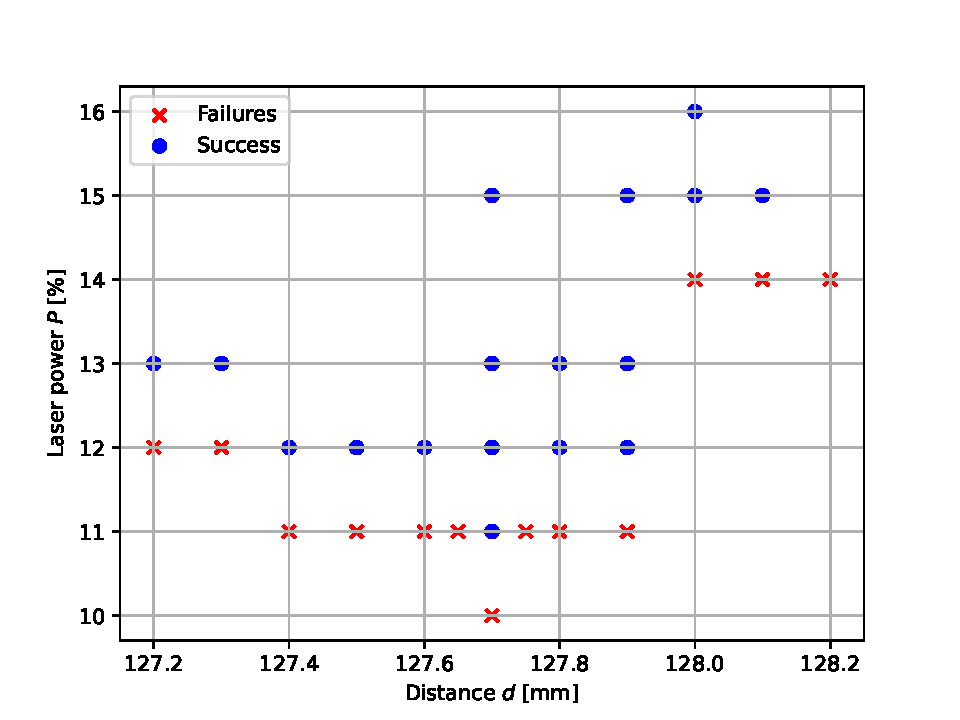
\includegraphics[width=0.75\textwidth]{assets/5 results/125mm_focus_threshold.pdf}
                \caption{125 mm focal length lens}
            \end{figure}
            
            Ignition at \qty{11}{\%} was attained once, but it was not possible to replicate this. A tighter focus was necessary to increase ignition reliability.

            % Graph of multi-lens
            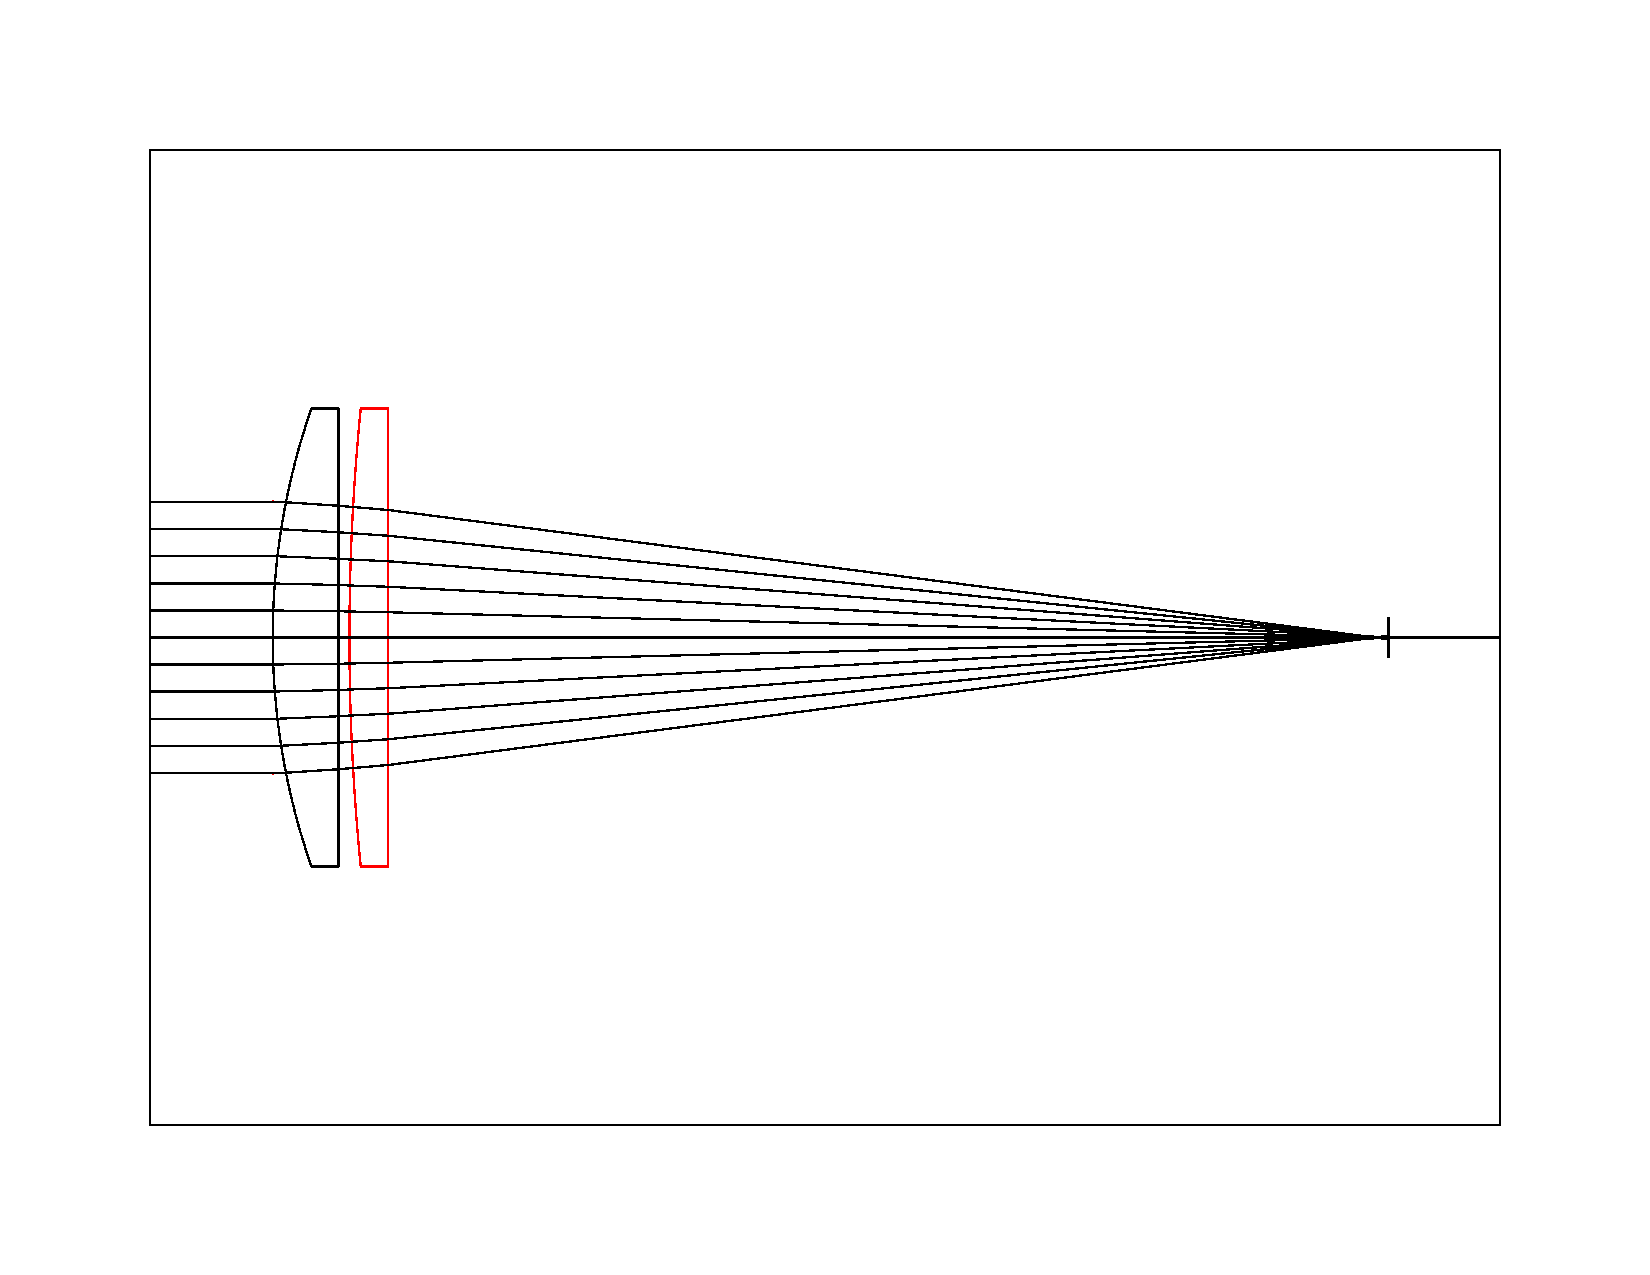
\includegraphics[width=\textwidth]{assets/5 results/500 and 150 lenses.pdf}

            \begin{figure}[h]
                \centering
                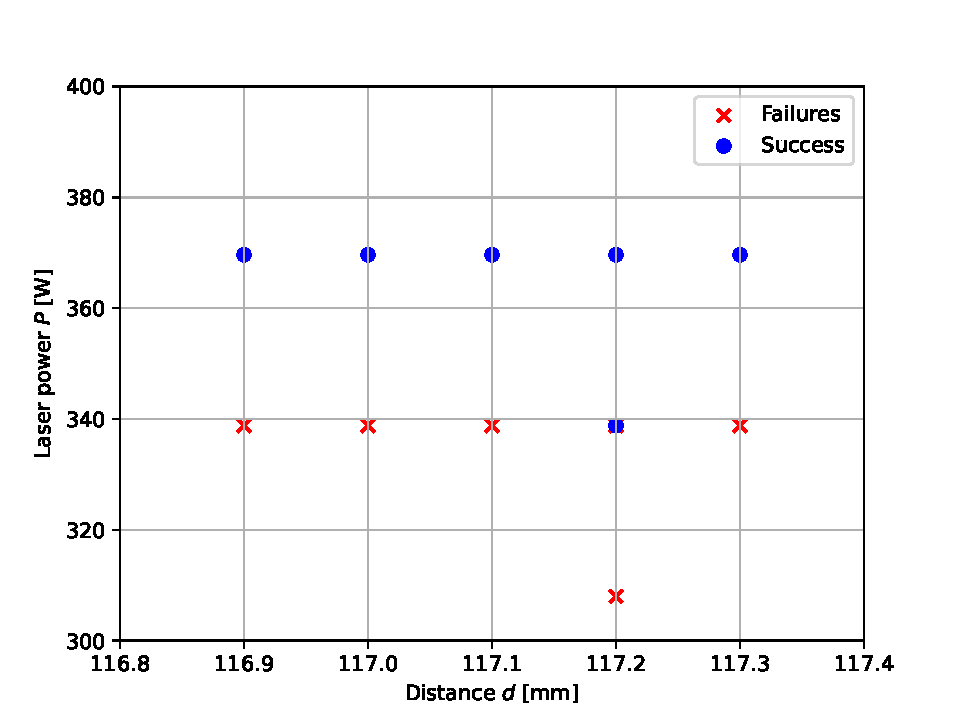
\includegraphics[width=0.75\textwidth]{assets/5 results/duallens_focus_threshold.pdf}
                \caption{Multi-lens system}
            \end{figure}

            % Section on power meter reading lower pulsed power at these low power settings, like about 200W

            The completion of these tests validated LSP generation in the CW power regime of the laser. The V2 thruster was then set up to ultimately test CW operation with flowing argon.

    \section{V2}
        This section presents the various experiments that were conducted with the V2 thruster.
    
        \subsection{Initial LSP shots}

            \begin{figure}
                \centering
                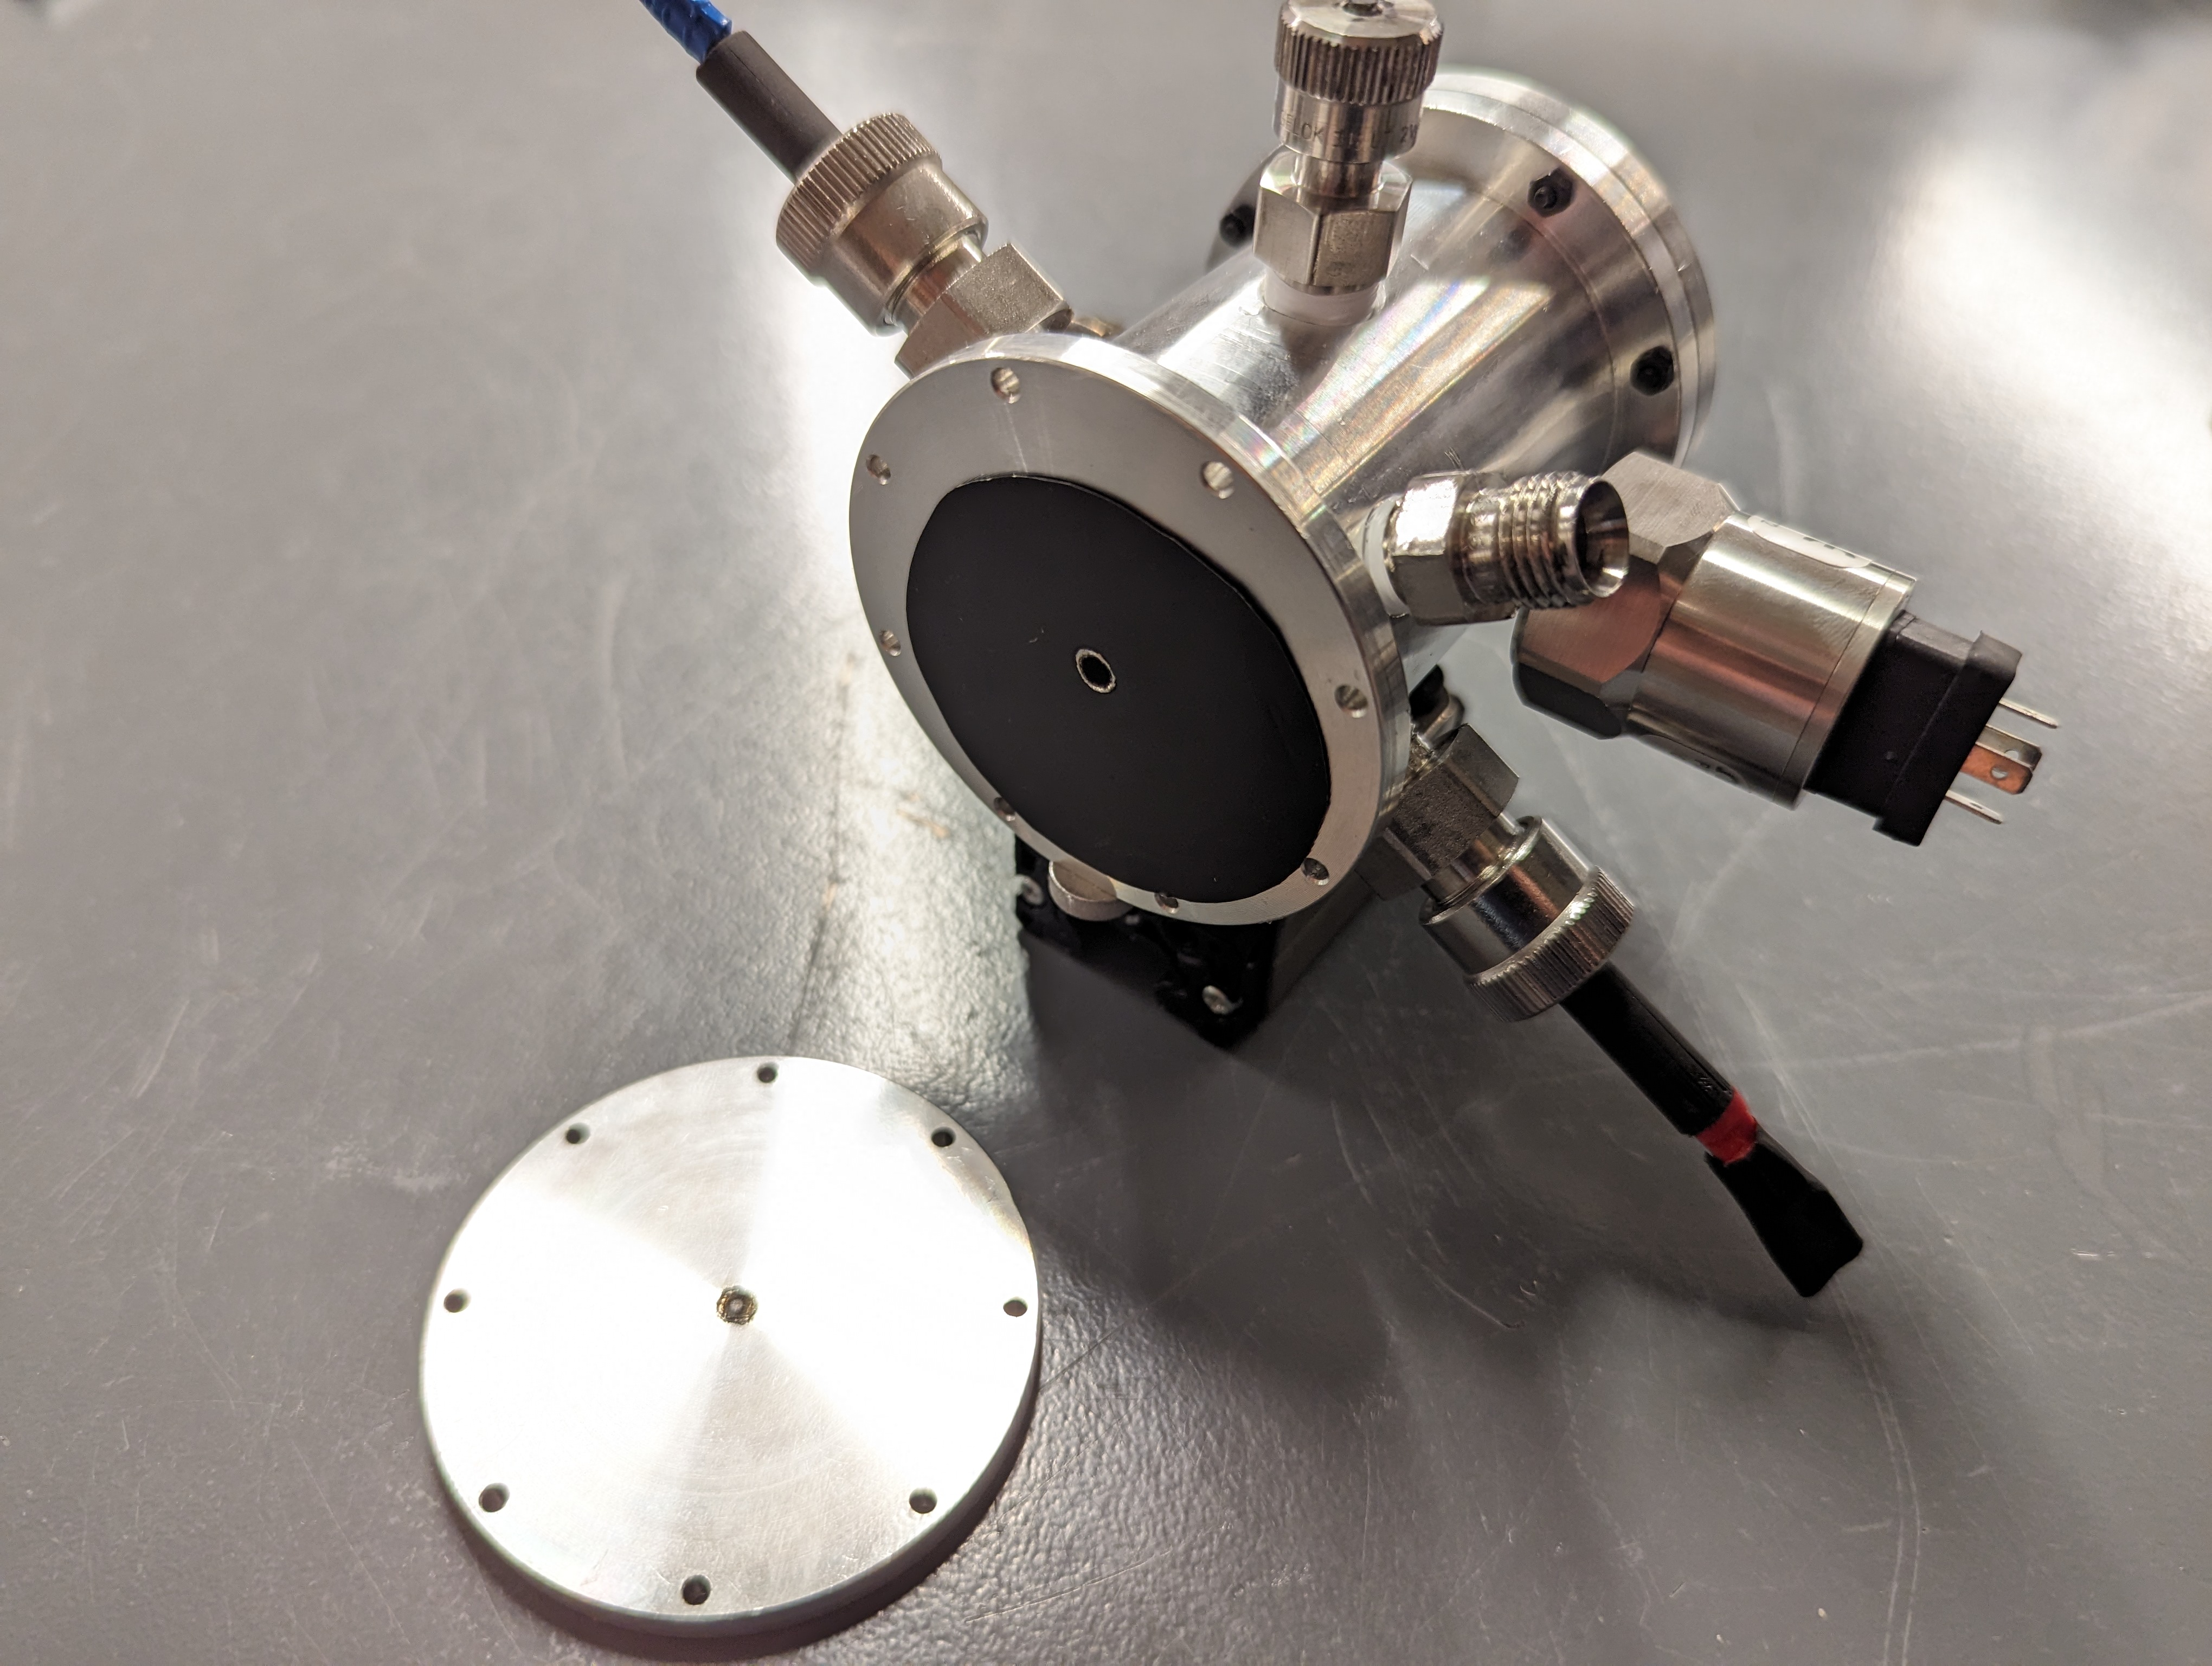
\includegraphics[width=0.75\textwidth]{assets/5 results/V2 test damage.jpg}
                \caption{Damage to the thruster after two \qty{3}{kW} laser shots}
            \end{figure}

            % Stills of first High-speed LSP video, showing expansion of LSP wave like in V1
        
        \subsection{Cold flow thrust tests}

            Cold flow tests were completed to give a baseline measurement of thrust before the hot fire test, and to validate the functioning of all data acquisition systems.
            
            % thrust vs pressure graph

        



